\documentclass[
BCOR 0.7cm,							% Bindekorrektur, bspw. 1 cm
11pt										% Schriftgroesse
]{scrbook}


\newif\ifpdf
\ifx\pdfoutput\undefined
	\pdffalse              	%normales LaTeX wird ausgef�hrt
\else
	\pdfoutput=1           
	\pdftrue               	%pdfLaTeX wird ausgef�hrt
\fi

\ifpdf %%Einbindung von Grafiken mittels \includegraphics{datei}
	\usepackage[pdftex]{graphicx} %%Grafiken in pdfLaTeX
\else
	\usepackage[dvips]{graphicx} %%Grafiken und normales LaTeX
\fi

\ifpdf
	\pdfinfo
	{
    /Author (Manfred Kindl)                                
    /Title (Abgabetool)     
    /Subject (Benutzerhandbuch Abgabetool Assistenz)                                    
    /Keywords (Abgabe Abgabetool FH-Complete Technikum-Wien)
	}
\else			
\fi

\usepackage{listings} \lstset{numbers=left, numberstyle=\tiny, numbersep=5pt}
\lstset{language=tex} 

\usepackage[pdftex,colorlinks=true,urlcolor=blue,linkcolor=blue]{hyperref}
\usepackage[ngerman]{babel}		%Deutsche Worttrennung
\usepackage[T1]{fontenc}
\usepackage[latin9]{inputenc}
\usepackage{makeidx} % Stichwortverzeichnis erstellen aus \index{} Eintr�gen
\usepackage{float}
\usepackage[small,bf]{caption}
\usepackage{fancyhdr}
\usepackage{amssymb,amsmath}
\usepackage{color}
\usepackage{hyperref} % Paket zum formatieren der Hyperlinks
\hypersetup{colorlinks=false} % Formatiert die internen Links nicht. Optionen siehe unter: http://en.wikibooks.org/wiki/LaTeX/Hyperlinks#Customization

\addtokomafont{chapter}{\color[rgb]{0.0,0.376,0.584}} %Schriftfarbe f�r Kapitel�berschriften
\addtokomafont{section}{\color[rgb]{0.0,0.376,0.584}} %Schriftfarbe f�r Kapitel�berschriften
\addtokomafont{subsection}{\color[rgb]{0.0,0.376,0.584}} %Schriftfarbe f�r Kapitel�berschriften


\renewcommand{\rmdefault}{phv} % Arial
\renewcommand{\sfdefault}{phv} % Arial

\makeindex

\graphicspath{{../../../../images/}}

\setlength{\tolerance}{2000}
\setlength{\parindent}{0pt}
\setlength{\parskip}{1ex plus 0.5ex minus 0.2ex}
\addtolength{\textheight}{2cm}
\addtolength{\headheight}{2pt}
\setlength{\captionmargin}{20pt}
\floatstyle{plain}
\floatname{example}{Example}

\newfloat{example}{hbtp}{loe}[chapter]
\floatplacement{figure}{hbtp}
\floatplacement{table}{htbp}

\newcommand{\dollar}{\char36}

\newenvironment{info}[1]{
    %\hspace{-10mm}
     \framebox[\textwidth][l]{
        \begin{minipage}{1,3cm}
        
\includegraphics[width=1cm]{icon_info}
        \end{minipage}
        \begin{minipage}{12cm}
        #1
        \end{minipage}
    }
}

\newenvironment{achtung}[1]{
    %\hspace{-10mm}
     \framebox[\textwidth][l]{
        \begin{minipage}{1,3cm}
        
\includegraphics[width=1cm]{icon_achtung}
        \end{minipage}
        \begin{minipage}{12cm}
        #1
        \end{minipage}
    }    
}

\newenvironment{halt}[1]{
    %\hspace{-10mm}
     \framebox[\textwidth][l]{
        \begin{minipage}{1,3cm}
        
\includegraphics[width=1cm]{icon_halt}
        \end{minipage}
        \begin{minipage}{12cm}
        #1
        \end{minipage}
    }
}

\newenvironment{idee}[1] {
    %\hspace{-10mm}
     \framebox[\textwidth][l]{
        \begin{minipage}{1,3cm}
        
\includegraphics[width=1cm]{icon_idee}
        \end{minipage}
        \begin{minipage}{12cm}
        #1
        \end{minipage}
    }
}

\setlength{\unitlength}{1mm}

\newenvironment{markier}[5]
{    
    \thicklines \put(#2,#3){\vector(#4,#5){5}} \thinlines
    \put(#2,#3){\circle*{5}}
    \put(#2,#3){\textcolor{black}{\circle{5}}\makebox(-10,0){\textcolor{white}{#1}}}
}


\hyphenation{gleich-zeitig para-meter}


\begin{document}

\ifpdf
	\DeclareGraphicsExtensions{.pdf,.jpg,.png}
\else
	\DeclareGraphicsExtensions{.eps}
\fi

\pagestyle{fancyplain}
% Titelseite einbinden



\begin{titlepage}
\begin{center}

\vfill 
\includegraphics[width=0.7\textwidth]{fhcomplete}
\rule{1\textwidth}{1pt} % Horizontale Linie \rule{_Breite_}{_St�rke_} andersrum ist's vertikal

\vspace*{30mm} \Huge Abgabetool\\
%\vspace*{10mm}

\vfill 
\includegraphics[width=100mm]{cis}
\vspace*{10mm} 

\huge Handbuch f�r die Studiengangsassistenz\\

	
\large \vfill FH Technikum Wien\\

Wien, \today
\end{center}
\end{titlepage}





\tableofcontents			% Inhaltsverzeichnis

\frontmatter					% Vorspann (z.B. r�mische Seitenzahlen)

\chapter{Einleitung}
\label{Kapitel Einleitung}

Dieses Handbuch erl�utert die Benutzung und Funktion der Bachelor- und Diplomarbeitsabgabe (kurz Abgabetool) auf der CIS-Seite der FH Technikum Wien.

Das Abgabetool dient zur Interaktion zwischen LektorInnen und Studierenden rund um die Abgabe von Projektarbeiten (Bakk- bzw Diplomarbeiten).
Studierende haben die M�glichkeit, zu definierten Terminen Dokumente hochzuladen.\\
Lektoren k�nnen Abgabetermine (f�r einzelne oder mehrere Studierende) und Abgabefristen definieren und hochgeladene Dokumente betrachten und bewerten.



\mainmatter						% Hauptteil

%% Kapitel Anfang %%%%%%%%%%%%%%%%%%%%%%%%%%%%%%%%%%%%%%%%%%%%%%%%%


\chapter{Abgabetool f�r die Studiengangsassistenz}
\label{Kapitel Aufruf}
Der Aufruf der Assistenzoberfl�che erfolgt im FAS �ber \textit{Extras/Projektarbeitstermine}.

\begin {figure}
	\centering
	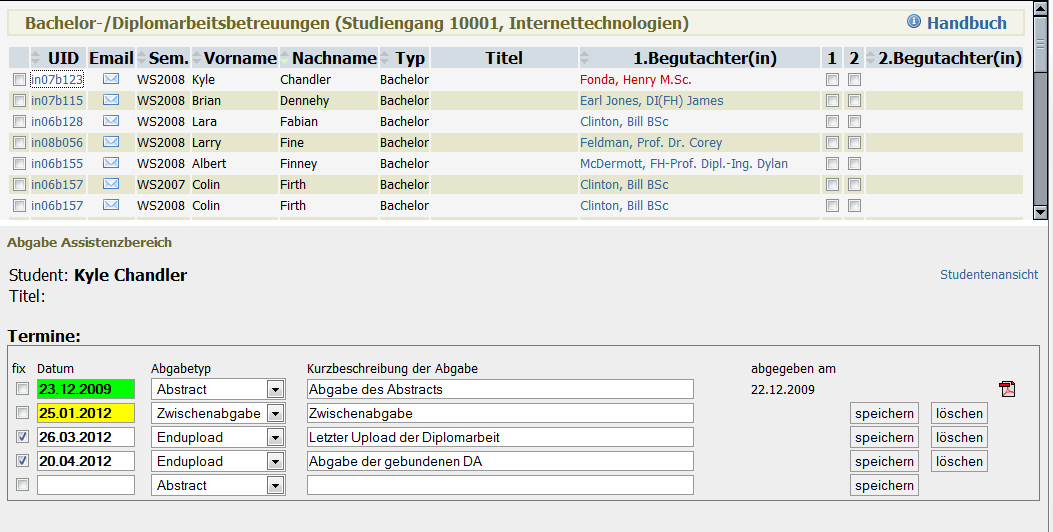
\includegraphics[width=1.0\textwidth]{abgabetool_uebersichtsliste_assistenz}
	\caption{Assistenzoberfl�che der Projektabgaben}
	\label{abgabetool_uebersichtsliste_assistenz}
\end {figure}

\section{�bersichtsliste der Betreuungen}
In der �bersichtsliste (siehe Abbildung \ref{abgabetool_uebersichtsliste_assistenz}) finden sich alle Betreuungen von Bachelor- und Diplomarbeiten (im FAS unter Projektarbeit als �berbegriff zusammengefasst, daher der Name Projektarbeitsabgabe), deren Autorin oder Autor noch aktiv sind.

\subsection{Aufrufen der Termin�bersicht}
Durch Anklicken der UID der Studentin/des Studenten in der zweiten Spalte der �bersichtsliste werden die Termindetails im unteren Teil der Seite angezeigt.

\subsection{E-Mail an einzelne Studierende}
Durch Anklicken des Briefsymbols in der dritten Spalte wird der E-Mailclient ge�ffnet und die Empf�nger- und Absenderadresse sowie \textit{Bachelorarbeitsbetreuung} bzw. \textit{Diplomarbeitsbetreuung} als Betreff werden vorausgef�llt.

\subsection{E-Mail an mehrere Studierende}
Um ein E-Mail an mehrere Studierende zu versenden, m�ssen zuerst die Studierenden durch Anklicken der Checkbox in der \textbf{ersten Spalte} markiert werden. Ein Klick auf den Button \textit{E-Mail Studierende} �ffnet den E-Mail-Client vorausgef�llt mit den E-Mailadressen der Auswahl.

\subsection{E-Mail an mehrere Begutachterinnen und Begutachter}
Um ein E-Mail an mehrere Begutachterinnen und Begutachter zu versenden, m�ssen diese durch Anklicken der Checkboxen in den Spalten \textit{1} bzw. \textit{2}, die sich zwischen den Spalten 1. Begutachter(in) und 2. Begutachter(in) befinden, markiert werden. Ein Klick auf den Button E-Mail Begutachter(innen) �ffnet den E-Mail-Client vorausgef�llt mit den EMailadressen der Auswahl.

\subsection{Termin f�r mehrere Studierende ansetzen}
Es gibt auch die M�glichkeit, f�r mehrere Studentinnen und Studenten Termine zu setzen. Dazu m�ssen zuerst die betreffenden Zeilen durch Anklicken der Checkbox in der ersten Spalte markiert werden. Danach �ffnet ein Klick auf den Button \textit{Terminserie anlegen} eine Eingabemaske im unteren Teil des Browserfensters. Hier wird dann ein Termin in die leere Zeile eingegeben. Der korrekte Abgabetyp mu� ausgew�hlt werden. Danach kann durch Dr�cken des Buttons \textit{+} eine weitere Zeile f�r einen neuen Termin erzeugt oder durch Dr�cken auf \textit{speichern} die bereits eingegebenen Termine f�r alle zuvor markierten Betreuungen gespeichert werden.

Die drei Buttons \textit{Terminserie anlegen}, \textit{E-Mail Studierende} und \textit{E-Mail Begutachter(innen)} befinden sich am unteren Ende der Liste der Betreuungen.

\subsection{Handbuch aufrufen}
Rechts neben der �berschrift \textit{Bachelor- /Diplomarbeitsbetreuungen} befindet sich der Link zum Handbuch. Durch einfaches Klicken darauf kann diese Anleitung als pdf-Datei aufgerufen werden.

\section{Termin�bersicht}

\subsection{Termineingabe und -bearbeitung}

\begin{itemize}
	\item Termineingabe: Die unterste Zeile der Liste ist bis auf das Auswahlfeld \textit{Abgabetyp} leer und f�r die Eingabe eines neuen Termins vorgesehen. Geben Sie ein Datum ein, w�hlen Sie den Abgabetyp aus und geben Sie eine kurze Beschreibung der Abgabe ein. Abschlie�end wird mit einem Klick auf den Button \textit{speichern} der Termin eingetragen.
	\item Termin�nderung: Termineintr�ge k�nnen ge�ndert werden, indem Sie die Daten der betreffenden Zeile �ndern und anschlie�end \textit{speichern} dr�cken.
	\item Termin l�schen: Termin k�nnen durch Klicken auf die Taste \textit{l�schen} gel�scht werden. Ist bereits eine Abgabe erfolgt, kann ein Termin nicht mehr gel�scht werden.
	
	\achtung{�ber alle drei Aktionen wird die Studentin/der Student per Mail informiert}
	\item Die Assistenz kann fixe Termine vergeben, erkennbar an dem roten Bullet unter \textit{fix}. Liegt ein Termin in der Vergangenheit, kann die Studentin/der Student zu diesem nichts mehr hochladen. Soll dennoch etwas hochgeladen werden, mu� die Studentin/der Student bei der Studiengangsassistenz um eine Korrektur des Termins ansuchen.
	
	\info{Es k�nnen nur selbst angelegte Termine ge�ndert und gel�scht werden}
\end{itemize}

\subsection{Farbcode}

\begin{itemize}
	\item wei�:	"`normaler"' Termin
	\item gelb:	Termin innerhalb der n�chsten 12 Tage
	\item rot:	Termin �berschritten
	\item gr�n:	Abgabe erfolgt
	\item hellrot: Abgabe nach Termin 
\end{itemize}

\subsection{Download der Abgabe und Ansicht der Zusatzdaten}
Durch Klicken auf das Symbol 
\includegraphics{icon_pdf} wird ein Dialogfenster zum Speichern oder Betrachten der Abgabe dieses Termins ge�ffnet.
Bei der Endabgabe m�ssen von der Studentin/dem Studenten zus�tzlich Daten f�r die Publikationsdatenbank eingegeben werden. Diese sollten mittels dem Symbol 
\includegraphics{icon_ordner_endabgabe} vor der Benotung �berpr�ft werden.

\subsection{Studentenansicht}
Sie k�nnen sich die Abgaben aus der Sicht der Studierenden ansehen. Klicken Sie dazu in der �bersichtsliste auf eine/n der Studierenden. Im unteren Teil des Fensters wird rechts der Button Studentenansicht angezeigt. Die Ansicht der/des Studierenden wird hier in einem neuen Fenster ge�ffnet. Falls Sie ein Fenster zur Passworteingabe erhalten, tragen Sie hier bitte Ihr eigenes Passwort und Ihren eigenen Benutzernamen ein.


%% Kapitel Ende   %%%%%%%%%%%%%%%%%%%%%%%%%%%%%%%%%%%%%%%%%%%%%%%%%
\appendix							% Beginn des Anhangs
%\chapter{Schluss}
%\listoftables				% Tabellenverzeichnis
%\listoffigures				% Abbildungsverzeichnis

\end{document}
